\documentclass[a4paper,10pt,oneside,openany]{jsbook}

\bibliographystyle{junsrt}  % 電子情報通信学会の論文誌スタイルになってる
\usepackage{amsmath,amssymb}
\usepackage{bm}
% \usepackage{epsbox}  %図表貼りつけ関連.epsファイルを扱う
\usepackage[dvipdfmx]{graphicx}
\usepackage[dvipdfmx]{color}
\usepackage{verbatim}
\usepackage{wrapfig}
\usepackage{ascmac}
\usepackage{makeidx}
\usepackage{here}
%subcaption ON
\usepackage[hang,small,bf]{caption}
\usepackage[subrefformat=parens]{subcaption}
\captionsetup{compatibility=false}
%tableに色つけ
\usepackage{colortbl}
%図とかの位置 H
\usepackage{here}

% セクション、サブセクションの文字の大きさ
\makeatletter
\def\@makechapterhead#1{
\vspace*{2\Cvs}
{\parindent \z@ \raggedright \normalfont
\Huge\headfont
\ifnum \c@secnumdepth >\m@ne
\if@mainmatter
\@chapapp\thechapter\@chappos
\hskip1zw
\fi
\fi
#1\par\nobreak
\vskip 3\Cvs}}
\makeatother

\makeindex
% 余白・文字数調整(左30mm, 右20mm, 上下共30mm, 文字数約40字/行, 行数約32行)
\setlength{\textwidth}{160truemm}      % テキスト幅: 210-(30+20)=160mm
\setlength{\fullwidth}{\textwidth}     % ページ全体の幅
\setlength{\oddsidemargin}{30truemm}   % 左余白
\addtolength{\oddsidemargin}{-1truein} % 左位置デフォルトから-1inch
\setlength{\topmargin}{30truemm}       % 上余白
\setlength{\textheight}{237truemm}     % テキスト高さ: 297-(30+30)=237mm
\addtolength{\topmargin}{-1truein}     % 上位置デフォルトから-1inch
\makeatother
\begin{document}
	% タイトル設定
	\thispagestyle{empty}
\begin{center}
	{\Huge 手指使用量の常時計測のためのウェアラブルデバイスの開発}\\
	\vspace{2mm}
	{\Large A wearable device for continuous monitoring of fingers activity}\\
	\vspace{7mm}
	{\Huge 松本 崇斗}\\
	\vspace{2mm}
	{\Large Takato MATSUMOTO}\\
	\vspace{10mm}
	{\Large (2017年度入学, 17646137)}\\
	\vspace{25mm}

	\begin{figure}[H]
		\begin{center}
			\vspace{7mm}
			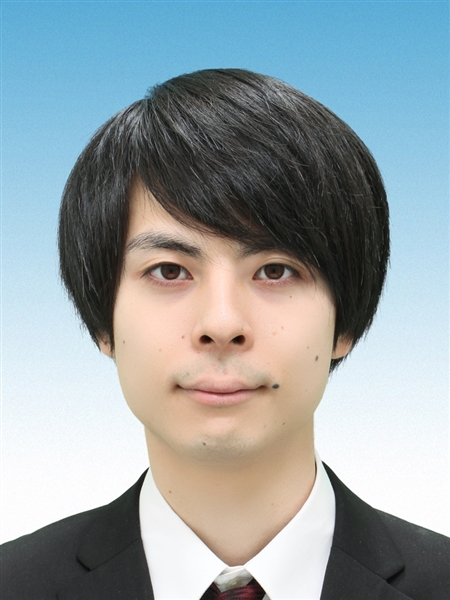
\includegraphics[width=45mm]{face_photo.jpg}
		\end{center}
	\end{figure}

	\vspace{25mm}
	{\Huge 指導教員 近藤敏之 教授}\\
	\vspace{12mm}
	{\Large 東京農工大学 工学府 情報工学専攻}\\
	\vspace{2mm}
	{\Large 2018年度修士論文}\\
	\vspace{2mm}
	{\Large (2018年1月30日 提出)}\\
\end{center}
	\frontmatter
	% 論文要旨
	\thispagestyle{empty}
\begin{center}
	{\large 東京農工大学 工学府 情報工学専攻 2018年度 修士論文 要旨}\\
	\vspace{8mm}
	{\Large 題目 手指使用量の常時計測のためのウェアラブルデバイスの開発}\\
	\vspace{2mm}
	{\large A wearable device for continuous monitoring of fingers activity}\\
	\vspace{8mm}
	{\large 学籍番号 17646137  氏名 松本 崇斗 (Takato MATSUMOTO)}\\
	\vspace{2mm}
	{\large 提出日 2018年1月30日}\\
	\vspace{4mm}
\end{center}














	% 目次
	\tableofcontents

	\mainmatter

	% 第1章 序論
	\chapter{序論}

\section{はじめに}
\label{1-1}



\section{本論文の構成}

	% 第2章 背景
	\chapter{理論}

\section{}
\label{model}



	% 第3章 実験システム
	\chapter{実験システムと方法}





	% 第4章 結果
	\chapter{実験結果}

	% 第5章
	\chapter{考察と課題}

	% 第6章
	%\chapter{考察と課題}


	% 付録
	% \appendix
	% \include{appendixA}
	% \include{appendixB}

	% 謝辞
	\chapter*{謝辞}

	% 参考文献
	\bibliography{ref}

	\newpage
	\printindex
\end{document}